\chapter{Thực nghiệm}
\label{chap:thucnghiem}

Chương này gồm hai phần. Phần đầu trình bày thực nghiệm của bài báo gốc (Section~6 của~\cite{hardt2016train}). Phần sau trình bày thực nghiệm do nhóm tự thực hiện ở quy mô nhỏ, dùng đúng phương pháp đo của bài báo, để kiểm tra lại các nhận định lý thuyết của Chương~\ref{chap:coso} và Chương~\ref{chap:convexrisk}.

\section{Thực nghiệm của bài báo}
\label{sec:thucnghiem-baibao}

\subsection{Mục tiêu và phương pháp đo}

Các định lý ở Chương~\ref{chap:coso} là giới hạn trên. Thực nghiệm của bài báo không nhằm kiểm chứng giá trị số của các giới hạn này mà nhằm trả lời hai câu hỏi: (1) trên mạng nơ-ron thực tế, Generalization Gap có phụ thuộc vào learning rate và số bước huấn luyện theo đúng xu hướng lý thuyết dự đoán hay không; (2) khoảng cách tham số $\delta_t = \|w_t - w'_t\|$, đại lượng trung tâm của mọi chứng minh, có thực sự đi cùng chiều với Generalization Gap hay không.

Thủ tục đo mô phỏng trực tiếp định nghĩa Uniform Stability:
\begin{enumerate}
    \item Bỏ một mẫu ngẫu nhiên khỏi tập huấn luyện để được tập $S$.
    \item Thay một mẫu ngẫu nhiên của $S$ bằng mẫu vừa bỏ ra để được tập $S'$; $S$ và $S'$ khác nhau đúng một mẫu.
    \item Huấn luyện hai mô hình trên $S$ và $S'$ với cùng khởi tạo và cùng random seed, tức cùng thứ tự duyệt mẫu. Đây chính là kỹ thuật coupling trong chứng minh ở Mục~\ref{subsec:yydungminh}.
    \item Cứ sau một số bước, đo khoảng cách Euclid giữa hai bộ tham số; sau mỗi epoch, đo lỗi trên tập huấn luyện và tập kiểm tra.
\end{enumerate}

\subsection{Các bài toán thực nghiệm}

\begin{table}[H]
\centering
\caption{Các bài toán thực nghiệm trong bài báo.}
\label{tab:thucnghiem-baibao}
\begin{tabular}{|p{2.6cm}|p{6.4cm}|p{4.2cm}|}
\hline
\textbf{Dữ liệu} & \textbf{Mô hình và thiết lập} & \textbf{Kết quả trình bày} \\ \hline
CIFAR-10 & Mạng tích chập gồm ba lớp convolution, mỗi lớp theo sau bởi pooling; không dùng weight decay, dropout hay data augmentation; learning rate cố định; test error dưới 20\% & Hình 1 của bài báo: generalization error, khoảng cách tham số, so sánh hai đại lượng \\ \hline
MNIST & Mô hình kiểu LeNet: hai lớp convolution (20 và 50 đơn vị) và một lớp fully connected; minibatch 60 & Kết quả bổ sung trong bản đầy đủ (arXiv) của bài báo \\ \hline
ImageNet & Kiến trúc AlexNet chuẩn, có data augmentation, regularization và dropout & Hình 2 của bài báo: thay mẫu sớm hay muộn; ảnh hưởng của kích thước mô hình \\ \hline
Penn Treebank & LSTM hai lớp, 200 đơn vị mỗi lớp, unroll 20 bước, minibatch 20, không dropout & Hình 3 của bài báo: mạng hồi quy \\ \hline
\end{tabular}
\end{table}

\subsection{Các phát hiện chính}

Bài báo rút ra bốn phát hiện:
\begin{enumerate}
    \item \textbf{Giảm learning rate một nửa thì generalization error giảm khoảng một nửa}, cả khi đo bằng tỉ lệ lỗi lẫn cross-entropy. Điều này khớp với Định lý~3.7, nơi giới hạn tỉ lệ thuận với $\sum_t \alpha_t$.
    \item \textbf{Khoảng cách tham số tăng chậm hơn tuyến tính}, kể cả với mạng không lồi, trong khi lý thuyết (Bổ đề~3.6) cho phép khoảng cách tăng theo cấp số nhân. Các giới hạn lý thuyết vì vậy còn lỏng (chưa chặt) so với thực tế.
    \item \textbf{Khoảng cách tham số và generalization error di chuyển cùng nhau.} Đây là bằng chứng thực nghiệm rằng $\delta_t$ là đại lượng phù hợp để đo độ ổn định.
    \item \textbf{Thời điểm gặp mẫu khác biệt quan trọng.} Khi mẫu khác biệt được đặt ở bước đầu tiên, khoảng cách tham số tăng nhanh hơn hẳn so với khi nó xuất hiện muộn; hiện tượng rõ nhất trên ImageNet. Điều này xác nhận vai trò của burn-in period trong chứng minh Định lý~3.8.
\end{enumerate}
Ngoài ra, trên ImageNet không dùng data augmentation, bài báo ghi nhận kích thước mô hình chỉ ảnh hưởng thứ yếu đến generalization error so với learning rate.

\subsection{Nhận xét phản biện}

Thực nghiệm của bài báo minh họa xu hướng chứ không kiểm chứng giới hạn. Ba điểm cần lưu ý: thực nghiệm dùng learning rate cố định trong khi Định lý~3.8 yêu cầu $\alpha_t \le c/t$; khoảng cách được đo trên một cặp $(S, S')$ cụ thể trong khi Uniform Stability lấy cận trên trên mọi cặp; và mạng thực tế (ReLU, cross-entropy) không thỏa chặt chẽ giả thiết Lipschitz và Smoothness toàn cục.

\section{Thực nghiệm của nhóm}
\label{sec:thucnghiem-nhom}

\subsection{Thiết lập}

Nhóm tái hiện thủ tục đo của bài báo ở quy mô nhỏ để có thể chạy trên máy tính cá nhân trong khoảng một phút. Mã nguồn được mô tả ở Phụ lục~\ref{app:code}.
\begin{itemize}
    \item \textbf{Dữ liệu:} bộ chữ số viết tay $8\times 8$ của thư viện scikit-learn (1\,797 ảnh, 10 lớp, 64 đặc trưng, chuẩn hóa về $[0,1]$). Lấy $n = 1\,000$ ảnh làm tập huấn luyện và 796 ảnh làm tập kiểm tra.
    \item \textbf{Mô hình lồi:} hồi quy logistic đa lớp, hàm mất mát cross-entropy (lồi theo tham số).
    \item \textbf{Mô hình không lồi:} mạng một lớp ẩn 100 đơn vị, hàm kích hoạt $\tanh$ (trơn, nên gần với giả thiết $\beta$-smooth hơn ReLU).
    \item \textbf{SGD:} minibatch 1, duyệt theo hoán vị ngẫu nhiên mỗi epoch, learning rate cố định $\alpha \in \{0{,}025;\ 0{,}05;\ 0{,}1\}$, 30 epoch ($T = 30\,000$ bước).
    \item \textbf{Đo lường:} tạo $S, S'$ theo đúng thủ tục ở Mục~\ref{sec:thucnghiem-baibao}; đo $\delta_t$ sau mỗi 100 bước; đo Generalization Gap (loss test trừ loss train, và tỉ lệ lỗi test trừ tỉ lệ lỗi huấn luyện) sau mỗi epoch. Mọi kết quả là trung bình trên 5 cặp $(S, S')$ khác nhau.
\end{itemize}

\subsection{Ảnh hưởng của learning rate: trường hợp lồi}

\begin{figure}[H]
\centering
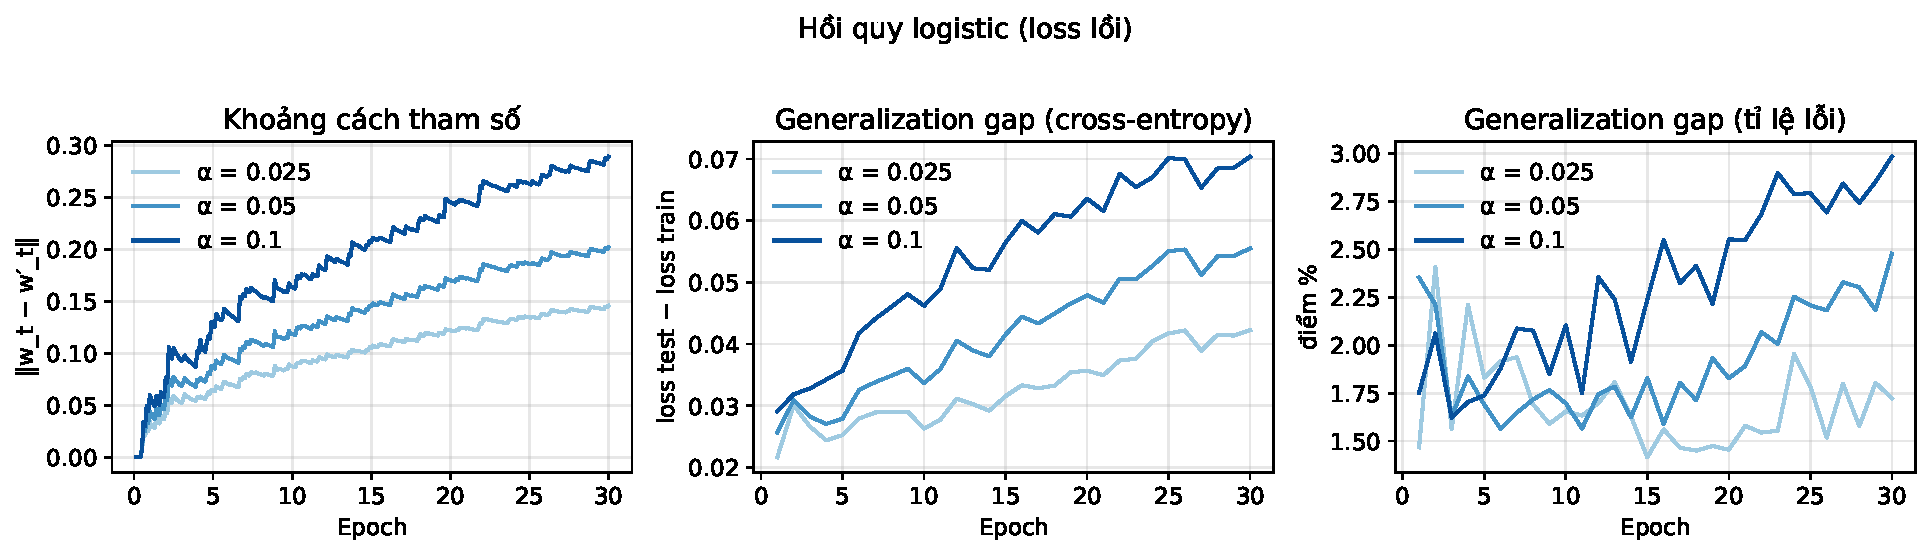
\includegraphics[width=\textwidth]{graphics/exp_convex_lr.pdf}
\caption{Hồi quy logistic: khoảng cách tham số và Generalization Gap theo epoch với ba mức learning rate.}
\label{fig:exp-convex}
\end{figure}

\begin{table}[H]
\centering
\caption{Kết quả sau 30 epoch, hồi quy logistic (trung bình 5 cặp $S, S'$).}
\label{tab:exp-convex}
\begin{tabular}{|c|c|c|c|c|c|}
\hline
$\alpha$ & $\|w_T - w'_T\|$ & Gap cross-entropy & Gap tỉ lệ lỗi & Lỗi train & Lỗi test \\ \hline
0,025 & 0,146 & 0,042 & 1,7 điểm \% & 2,0\% & 3,7\% \\ \hline
0,05 & 0,202 & 0,056 & 2,5 điểm \% & 1,0\% & 3,5\% \\ \hline
0,1 & 0,289 & 0,070 & 3,0 điểm \% & 0,7\% & 3,6\% \\ \hline
\end{tabular}
\end{table}

Hình~\ref{fig:exp-convex} và Bảng~\ref{tab:exp-convex} cho thấy:
\begin{itemize}
    \item Learning rate càng lớn thì khoảng cách tham số và Generalization Gap càng lớn, đúng xu hướng với Định lý~3.7. Lỗi test gần như không đổi (3,5--3,7\%) vì learning rate lớn giảm lỗi huấn luyện nhanh hơn nhưng đồng thời mở rộng gap.
    \item Khoảng cách tham số tăng chậm hơn tuyến tính theo số bước (đường cong lõm), và khi gấp đôi $\alpha$ thì khoảng cách chỉ tăng khoảng 1,4 lần thay vì 2 lần như giới hạn $2\alpha L^2 T/n$. Kết quả này khớp với phát hiện thứ hai của bài báo: giới hạn lý thuyết đúng xu hướng nhưng còn lỏng về độ lớn.
\end{itemize}

\subsection{Ảnh hưởng của learning rate: trường hợp không lồi}

\begin{figure}[H]
\centering
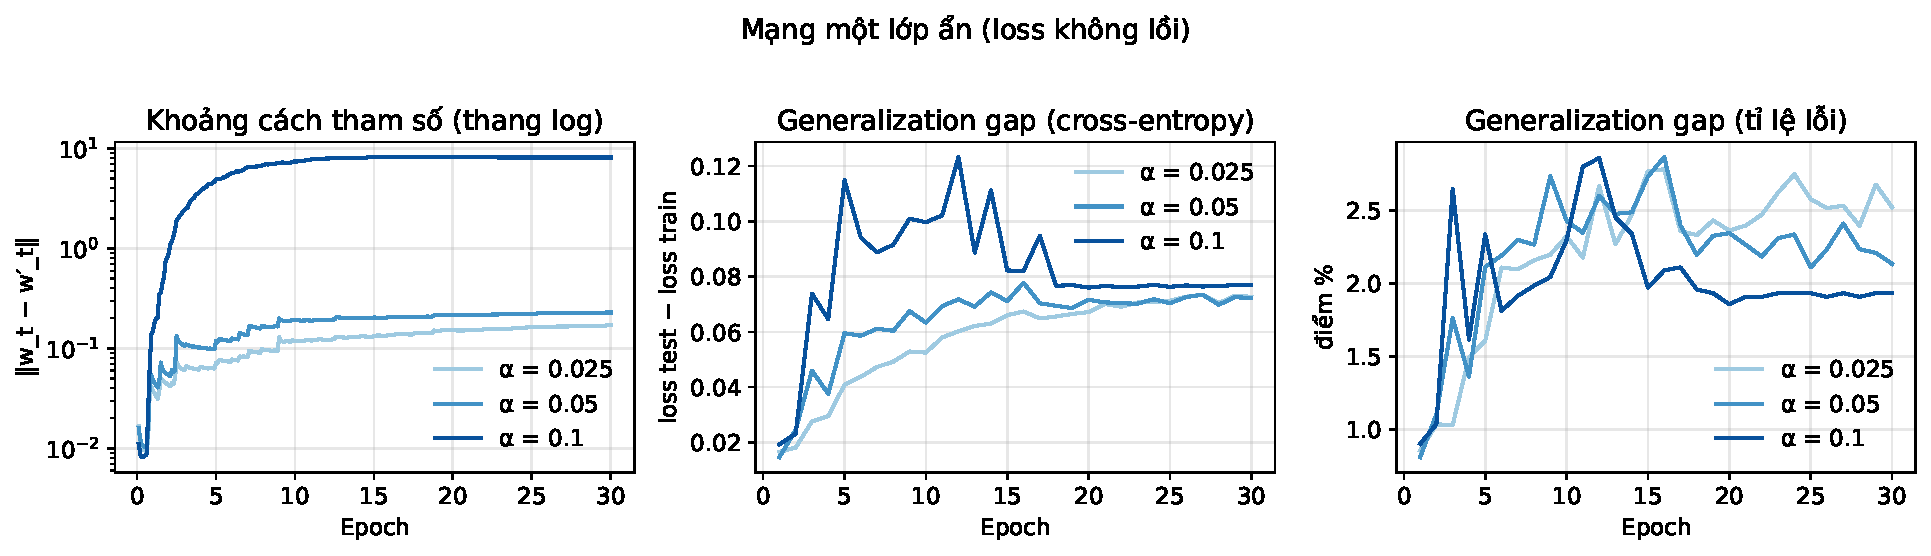
\includegraphics[width=\textwidth]{graphics/exp_nonconvex_lr.pdf}
\caption{Mạng một lớp ẩn: khoảng cách tham số (thang logarit) và Generalization Gap theo epoch với ba mức learning rate.}
\label{fig:exp-nonconvex}
\end{figure}

\begin{table}[H]
\centering
\caption{Kết quả sau 30 epoch, mạng một lớp ẩn (trung bình 5 cặp $S, S'$).}
\label{tab:exp-nonconvex}
\begin{tabular}{|c|c|c|c|c|c|}
\hline
$\alpha$ & $\|w_T - w'_T\|$ & Gap cross-entropy & Gap tỉ lệ lỗi & Lỗi train & Lỗi test \\ \hline
0,025 & 0,17 & 0,073 & 2,5 điểm \% & 0,04\% & 2,6\% \\ \hline
0,05 & 0,23 & 0,072 & 2,1 điểm \% & 0\% & 2,1\% \\ \hline
0,1 & 8,1 & 0,077 & 1,9 điểm \% & 0\% & 1,9\% \\ \hline
\end{tabular}
\end{table}

Trường hợp không lồi cho kết quả phức tạp hơn và cần đọc cẩn thận:
\begin{itemize}
    \item Với $\alpha = 0{,}025$ và $0{,}05$, khoảng cách tham số nhỏ và tăng chậm, tương tự trường hợp lồi.
    \item Với $\alpha = 0{,}1$, khoảng cách tham số tăng vọt lên khoảng 8 trong vài epoch đầu, ở cả 5 cặp $(S, S')$. Đây đúng là hiện tượng mà Bổ đề~3.6 cảnh báo: với hàm không lồi, quy tắc cập nhật là $(1 + \alpha\beta)$-expansive, nên khi $\alpha$ đủ lớn, một sai khác nhỏ ban đầu bị khuếch đại đến mức hai mô hình hội tụ về hai nghiệm khác hẳn nhau.
    \item Tuy vậy, Generalization Gap ở $\alpha = 0{,}1$ không lớn hơn đáng kể. Lý do: mạng nơ-ron có nhiều nghiệm tốt tương đương nhau (ví dụ hoán đổi vị trí các nơ-ron ẩn cho cùng một hàm dự đoán), nên hai bộ tham số cách xa nhau vẫn có thể cho loss gần như nhau. Khoảng cách tham số chỉ là một \emph{cận trên} cho độ lệch loss qua tính Lipschitz; khi cận này lỏng, nó không còn phản ánh đúng Generalization Gap.
    \item Mô hình đạt lỗi huấn luyện 0\% ở mọi learning rate, nên Generalization Gap ở đây bằng chính lỗi test. Đây là chế độ mà thực nghiệm nhãn ngẫu nhiên của Zhang và cộng sự~\cite{zhang2017understanding} sau này khai thác (Chương~\ref{chap:ketluan}).
\end{itemize}

\subsection{Khoảng cách tham số và Generalization Gap đi cùng nhau}

\begin{figure}[H]
\centering
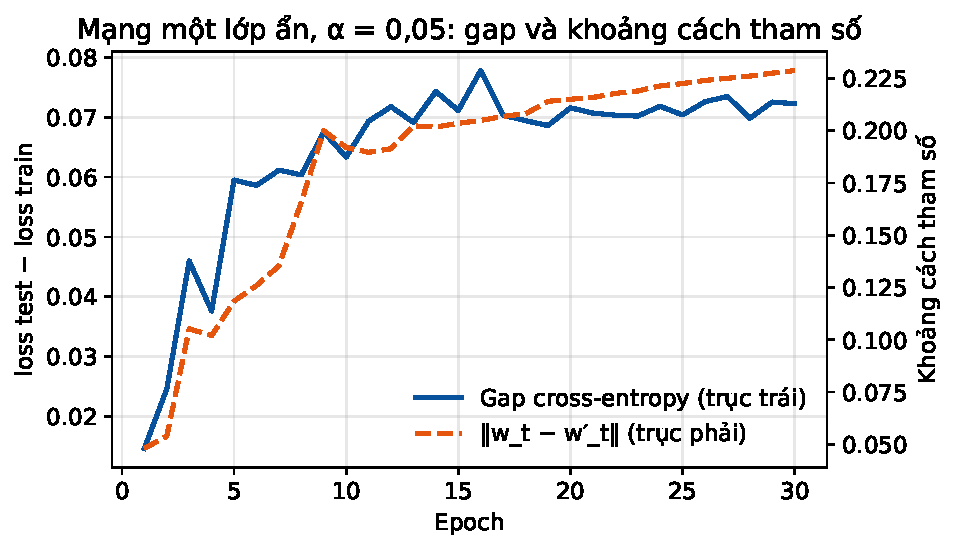
\includegraphics[width=0.75\textwidth]{graphics/exp_gap_vs_distance.pdf}
\caption{Mạng một lớp ẩn, $\alpha = 0{,}05$: Generalization Gap (cross-entropy, trục trái) và khoảng cách tham số (trục phải) theo epoch.}
\label{fig:exp-gap-distance}
\end{figure}

Trong chế độ learning rate vừa phải ($\alpha = 0{,}05$), hai đại lượng tăng gần như song song (Hình~\ref{fig:exp-gap-distance}); hệ số tương quan Pearson giữa khoảng cách tham số cuối mỗi epoch và gap cross-entropy là $0{,}93$. Kết quả này tái hiện phát hiện thứ ba của bài báo, với lưu ý rằng mối liên hệ bị phá vỡ khi learning rate quá lớn như đã thấy ở mục trước.

\subsection{Burn-in: thời điểm gặp mẫu khác biệt}

\begin{figure}[H]
\centering
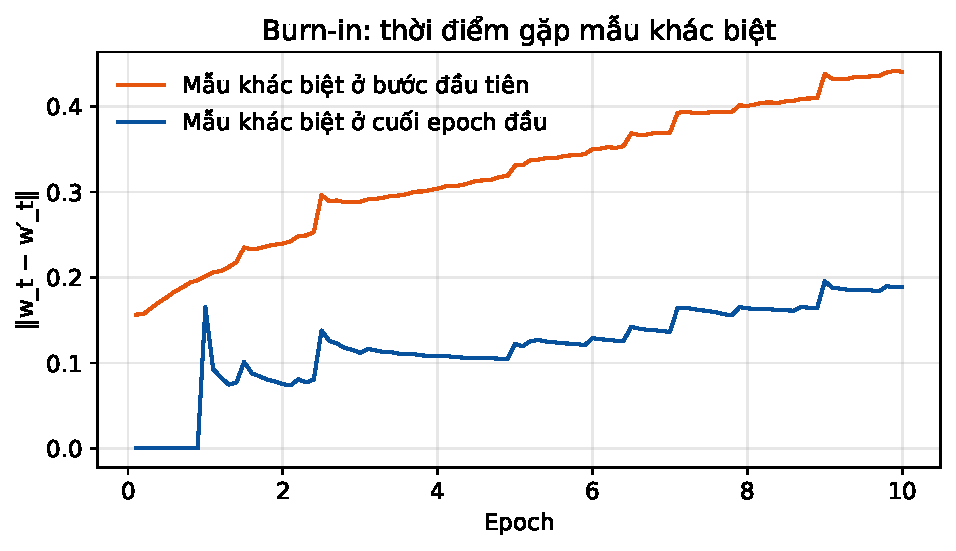
\includegraphics[width=0.75\textwidth]{graphics/exp_burnin.pdf}
\caption{Mạng một lớp ẩn, $\alpha = 0{,}05$: khoảng cách tham số khi mẫu khác biệt được duyệt ở bước đầu tiên so với ở cuối epoch đầu tiên.}
\label{fig:exp-burnin}
\end{figure}

Nhóm cố định vị trí của mẫu khác biệt trong hoán vị của epoch đầu tiên: ở bước đầu tiên, hoặc ở bước cuối cùng của epoch. Sau 10 epoch, khoảng cách tham số là $0{,}44$ khi mẫu khác biệt xuất hiện ngay bước đầu, so với $0{,}19$ khi nó xuất hiện ở cuối epoch đầu, tức lớn hơn khoảng 2,3 lần (Hình~\ref{fig:exp-burnin}). Khi hai quỹ đạo tách nhau sớm, lúc tham số còn ở vùng khởi tạo và mô hình đang thay đổi nhanh, sai khác có nhiều thời gian và nhiều ``động lực'' để bị khuếch đại. Kết quả này tái hiện phát hiện thứ tư của bài báo và minh họa trực tiếp lý do burn-in period là chìa khóa của Định lý~3.8.

\subsection{Weight Decay}

\begin{figure}[H]
\centering
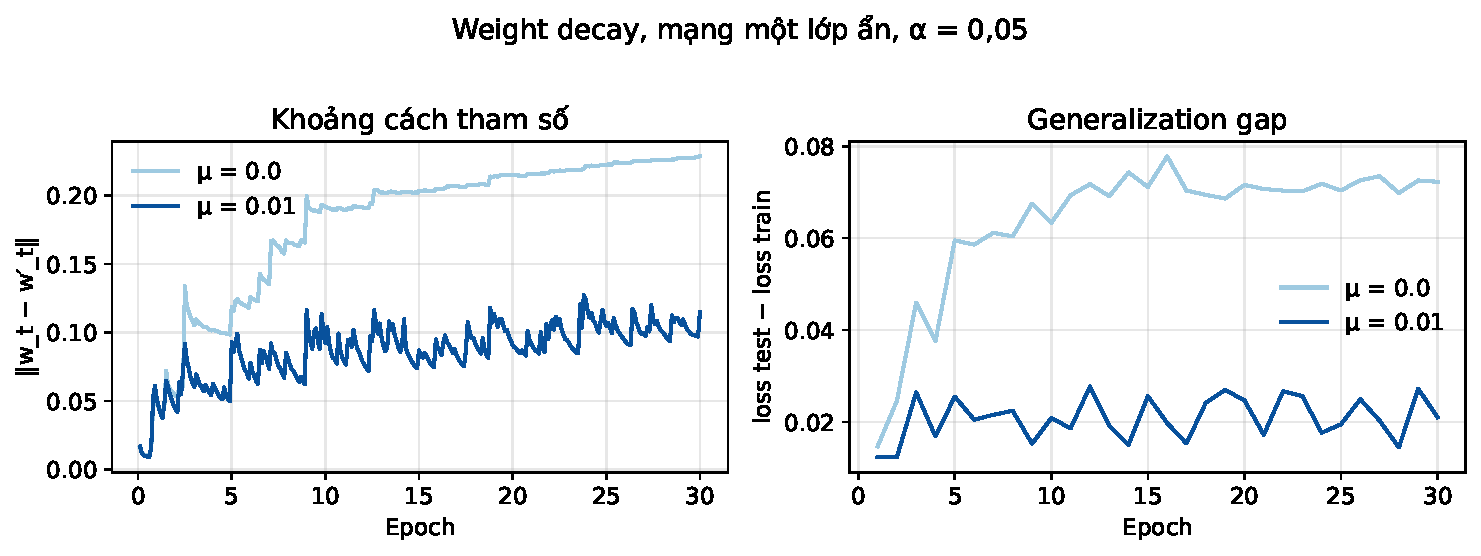
\includegraphics[width=0.9\textwidth]{graphics/exp_weight_decay.pdf}
\caption{Mạng một lớp ẩn, $\alpha = 0{,}05$: khoảng cách tham số và Generalization Gap khi không dùng và có dùng weight decay $\mu = 0{,}01$.}
\label{fig:exp-wd}
\end{figure}

Thêm weight decay $\mu = 0{,}01$ (mỗi bước nhân tham số với $1 - \alpha\mu$) làm khoảng cách tham số giảm khoảng một nửa (từ $0{,}23$ xuống $0{,}12$) và gap cross-entropy giảm từ $0{,}072$ xuống $0{,}021$, phù hợp với Bổ đề~4.2: weight decay giảm hệ số giãn nở từ $1 + \alpha\beta$ xuống $1 + \alpha(\beta - \mu)$. Tuy nhiên, lỗi huấn luyện tăng từ 0\% lên 5,8\% và lỗi test tăng từ 2,1\% lên 7,0\%. Đây đúng là sự đánh đổi ở Chương~\ref{chap:convexrisk}: tăng Stability (giảm $\epsilon_{\mathrm{stab}}$) có thể phải trả giá bằng sai số tối ưu ($\epsilon_{\mathrm{opt}}$) lớn hơn; mức $\mu$ phù hợp cần được chọn để cân bằng hai thành phần.

\subsection{Tổng hợp}

\begin{table}[H]
\centering
\caption{Đối chiếu thực nghiệm của nhóm với nhận định của bài báo.}
\label{tab:doichieu}
\begin{tabular}{|p{5.4cm}|p{4cm}|p{3.8cm}|}
\hline
\textbf{Nhận định của bài báo} & \textbf{Kết quả của nhóm} & \textbf{Mức độ khớp} \\ \hline
Learning rate nhỏ hơn cho gap nhỏ hơn (Định lý~3.7) & Đúng với hồi quy logistic; không rõ với mạng không lồi & Khớp ở trường hợp lồi \\ \hline
Khoảng cách tham số tăng chậm hơn tuyến tính & Đúng ở cả hai mô hình khi $\alpha \le 0{,}05$ & Khớp \\ \hline
Khoảng cách tham số đi cùng gap & Tương quan $0{,}93$ ở $\alpha = 0{,}05$; bị phá vỡ ở $\alpha = 0{,}1$ & Khớp một phần \\ \hline
Gặp mẫu khác biệt sớm làm khoảng cách tăng nhanh hơn & Lớn hơn khoảng 2,3 lần sau 10 epoch & Khớp \\ \hline
Weight decay làm tăng Stability (Bổ đề~4.2) & Khoảng cách giảm một nửa, gap giảm, lỗi test tăng & Khớp, kèm đánh đổi \\ \hline
\end{tabular}
\end{table}

\textbf{Hạn chế của thực nghiệm.} Dữ liệu và mô hình nhỏ hơn nhiều so với bài báo; learning rate cố định thay vì $c/t$; chỉ lấy trung bình trên 5 cặp $(S, S')$ nên các đường gap còn dao động. Các kết quả vì vậy chỉ có giá trị minh họa xu hướng, giống như thực nghiệm của bài báo gốc.
